\documentclass[10pt]{article} 
\usepackage{ctex}
\usepackage{graphicx}
\usepackage{amsmath}
\usepackage{epstopdf}
\usepackage{tabularx}
\usepackage{geometry}
\usepackage{float}
\usepackage{listings}
\usepackage{xcolor}
\usepackage{fontspec}
\usepackage{color}
\usepackage{caption}
\usepackage[dvipsnames]{xcolor}
\lstset{
	language = matlab,
	backgroundcolor = \color{yellow!10}, % 背景色:淡黄
	basicstyle = \small\ttfamily, % 基本样式 + 小号字体
	rulesepcolor= \color{gray}, % 代码块边框颜色
	breaklines = true, % 代码过长则换行
	numbers = left, % 行号在左侧显示
	numberstyle = \small, % 行号字体
	keywordstyle = \color{blue}, % 关键字颜色
	commentstyle =\color{green!60}, % 注释颜色
	stringstyle = \color{red!100}, % 字符串颜色
	frame = shadowbox, % 用(带影子效果)方框框住代码块
	showspaces = false, % 不显示空格
	columns = fixed, % 字间距固定
	%escapeinside={} % 特殊自定分隔符:
	morekeywords = {as}, % 自加新的关键字(必须前后都是空格)
	deletendkeywords = {compile} % 删除内定关键字;删除错误标记的关键字用deletekeywords删!
}
\geometry{right=1cm,left=1cm,top=1cm,bottom=1.5cm}
\makeatletter
\newcommand*\@lbracket{[}
\newcommand*\@rbracket{]}
\newcommand*\@colon{:}
\newcommand*\colorIndex{%
    \edef\@temp{\the\lst@token}%
    \ifx\@temp\@lbracket \color{black}%
    \else\ifx\@temp\@rbracket \color{black}%
    \else\ifx\@temp\@colon \color{black}%
    \else \color{vorange}%
    \fi\fi\fi
}
\makeatother
\usepackage{trace}
\title{语音合成大作业}
\author{王炜致\ 2022010542}
\date{}
\begin{document}
\maketitle
\section{语音预测模型}
\subsection*{(1)}
\textbf{
给定$$e(n) = s(n) - a_1s(n - 1) - a_2s(n - 2)$$
假设 e(n) 是输入信号, s(n) 是输出信号, 上述滤波器的传递函数是什么? 如果 $a_1 = 1.3789
$,$a_2 = -0.9506$,上述合成模型的共振峰频率是多少?用zplane , freqz , impz分别绘出零
极点图,频率响应和单位样值响应。用 filter 绘出单位样值响应,比较和 impz 的是否相同。}

\textcircled{1}上述滤波器的传播函数为$$H(z)=\frac{1}{1-\frac{a_1}{z}-\frac{a_2}{z^2}} 
=\frac{z^2}{z^2-a_1z-a_2}$$

\textcircled{2}共振峰频率$$f=\frac{\omega}{2\pi}$$
而模拟频率$\omega$和数字频率$\Omega$有关系$$\Omega=\omega T$$
故$$f=\frac{\Omega}{2\pi T}\approx1kHz$$

\textcircled{3}用zplane,freqz分别绘出零极点图、频率响应
如下:
\begin{figure}[htbp]
	\centering
	\begin{minipage}{0.49\linewidth}
		\centering
		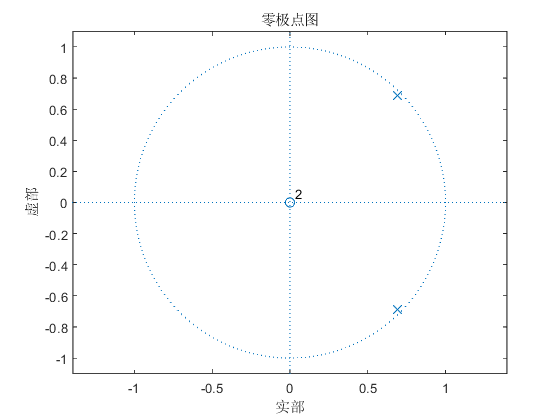
\includegraphics[width=0.9\linewidth]{drawing1-1.png}
		\caption{零极点图}
	\end{minipage}
	\begin{minipage}{0.49\linewidth}
		\centering
		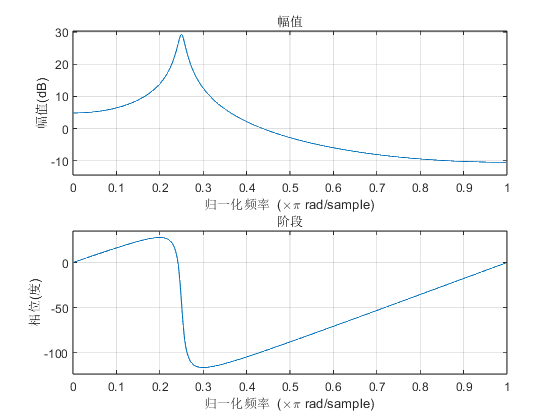
\includegraphics[width=0.9\linewidth]{drawing1-2.png}
		\caption{频率响应}
	\end{minipage}
	%\qquad
	%让图片换行,
\end{figure}

用impz,filter分别绘出单位样值响应如下,两者相同:
\begin{figure}[h]
	\centering
	\begin{minipage}{0.49\linewidth}
		\centering
		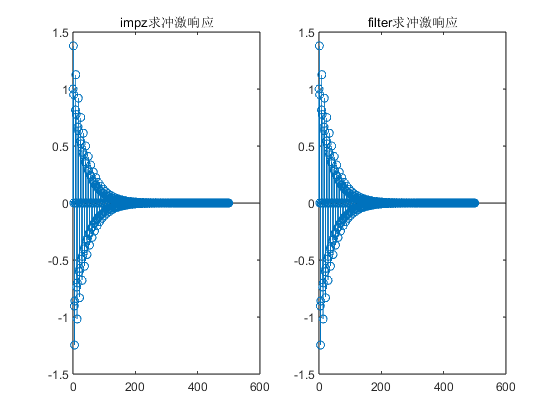
\includegraphics[width=0.9\linewidth]{drawing1-3.png}
		\caption{冲激响应}
	\end{minipage}
\end{figure}
\newpage
\subsection*{(3)((2)略)}
\textbf{运行程序到 27 帧时停住, 用(1) 中的方法观察零极点图。}

如下所示,用zplane函数绘制E,A决定的零极点图即可。
\begin{lstlisting}[language=matlab]
% (3) 在此位置写程序,观察预测系统的零极点图
    zplane(E,A);
    \end{lstlisting}

\begin{figure}[h]
	\centering
	\begin{minipage}{0.49\linewidth}
		\centering
		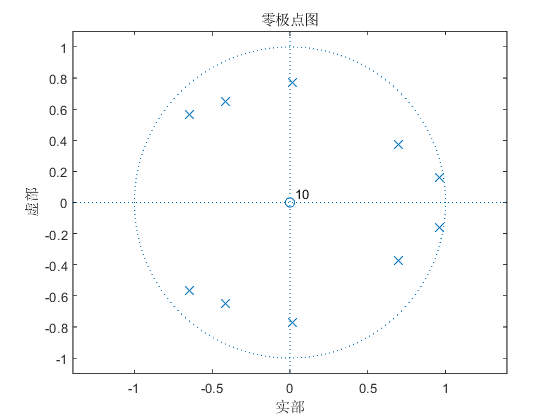
\includegraphics[width=0.9\linewidth]{coding1.png}
		\caption{27帧对应零极点图}
	\end{minipage}
\end{figure}

\subsection*{(4)}
\textbf{在循环中添加程序: 对每帧语音信号 s(n) 和预测模型系数 $\{a_i\} $, 用 filter 计算
激励信号 e(n) 。}

由于分帧处理,需要保存滤波器的最终条件zf,且需要考虑滤波器的初始状态zi,在代码中表现为更新zi\_pre
的值。
\begin{lstlisting}[language=matlab]
% (4) 在此位置写程序,用filter函数s_f计算激励,注意保持滤波器状态
    [exc_ftr,zi_pre] = filter(A,1,s_f,zi_pre);
    exc((n-1)*FL+1:n*FL) = exc_ftr;
% exc((n-1)*FL+1:n*FL) = ... 将你计算得到的激励写在这里
\end{lstlisting}
\subsection*{(5)}
\textbf{完善 speechproc.m 程序, 在循环中添加程序: 用你计算得到的激励信号 e(n) 和预
测模型系数 $\{a_i\} $ , 用 filter 计算重建语音 $\hat{s}(n)$ 。}

类似地有:
\begin{lstlisting}[language=matlab]
% (5) 在此位置写程序,用filter函数和exc重建语音,注意保持滤波器状态
    [rec_ftr,zi_rec] = filter(1,A,exc_ftr,zi_rec);
    s_rec((n-1)*FL+1:n*FL) = rec_ftr;
% s_rec((n-1)*FL+1:n*FL) = ... 将你计算得到的重建语音写在这里
\end{lstlisting}

\subsection*{(6)}
\textbf{在循环结束后添加程序: 用 sound 试听(6) 中的 e(n) 信号, 比较和 s(n) 以及 $\hat{s}(n)$
信号有何区别。 对比画出三个信号, 选择一小段, 看看有何区别。}

三个信号载有的信息均为“电灯比油灯进步多了”。
e(n)信号噪声较大;s(n)信号和$\hat{s}(n)$信号听起来几乎没有区别,且两者噪声相对e(n)较小。
\begin{figure}[h]
	\centering
	\begin{minipage}{0.49\linewidth}
		\centering
		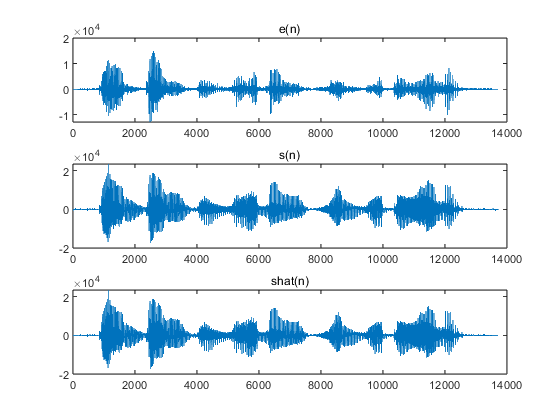
\includegraphics[width=0.9\linewidth]{compare.png}
		\caption{语音信号比较}
	\end{minipage}
\end{figure}

选取[2000,4000]局部区间比较:
\begin{figure}[h]
	\centering
	\begin{minipage}{0.49\linewidth}
		\centering
		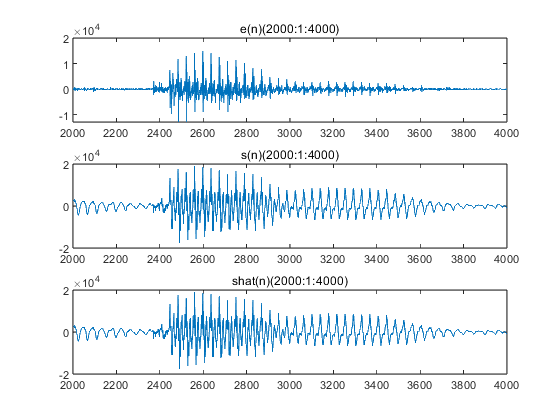
\includegraphics[width=0.9\linewidth]{commpare.png}
		\caption{语音信号比较(局部)}
	\end{minipage}
\end{figure}
进一步验证了前述判断。
\section{语音合成模型}
\subsection*{(7)}
\textbf{生成一个 8kHz 抽样的持续 1 秒钟的数字信号, 该信号是一个频率为 200Hz 的单
位样值“串”, 即$$x(n)=\sum_{i=0}^{NS-1}\delta(n-iN)$$考虑该信号的 N 和 NS 分别为何值? 
用 sound 试听这个声音信号。 再生成一个 300Hz 的单位样值“串”并试听, 有何区别? }
$$N=\frac{1}{8kHz}=1.25\times10^{-4}$$
\end{document}